\chapter{Premilinaries and Problem Definition}
\label{ch:premAndDef}


\section{The Friedkin and Johnsen Model}
\label{sec:prem}

The model will use the information about the opinion of the user, internal and external, but also the constant update of the external opinions of the neighbourhood of the user e.g. the friend list or the accounts the user follows
to compute an opinion vector. This vector is a metric for the whole social graph that can give us insight about its current situation. The vector values range from [-1,1]. Values closer to the range limits indicate bigger polarization. Polarized graphs create groups of nodes that are strongly connected with each other and feedback to one another the same extreme opinion over a topic. These groups can be seen clearly in the illustration of filter bubbles and often associated with politics and controversial issues of our society. Using a certain number of users we can achieve a reduction on the polarization of the network. 
\\
\\
\\
We can educate a group of users with the opposite view, and in terms of our model that means that we can modify the social graph by adding a connection between  users of different opinions. \\
\\
Let $G = (V,E)$ be a connected undirected graph representing a network. Let $z$ be the vector of expressed opinions  for the whole network. Each value  of the vector represents a node and can be computed with the opinion-formation model of Friedkin and Johnsen as follows. 

\begin{equation} 
	z_i = \frac{w_{ii}*si + \sum_{j \epsilon N(i) }{w_{ij}*z_j}} {w_{ii} + \sum_{j \epsilon N(i) }{w_{ij}}} 
\end{equation} 
\\
Where $s_i$ denotes the internal and $z_i$ the expressed opinion of a user. The internal opinion of a user corresponds to the views that inherently has for a controversial topic while the expressed one is the views that the user shares on a social network with his neighbours. The length of the opinion vector $||z|| ^2$ measures  the polarization of the network. To make the polarization  independent of its network we can  normalize it  by dividing  it with the length of the vector $z$. 
An equivalent way of obtaining the vector $z$ from a graph is the following: if $L$ is the laplacian matrix of a graph $G=(V,E)$, and $I$ is the identity matrix, then $z=(L+I)^{-1}S$ \cite{bindel}. 

\section{Measuring the polarization}
\label{sec:meas}

We measure the polarization by its distance from a neutral opinion. We can quantify this with the length of the vector of the second norm $L_{2}^2$ \cite{tsapMatakosTerzi}.

\begin{equation}
	\pi(z) = ||z||_{2}^2
\end{equation}
\\
This value can be independent of the network if we normalize it by dividing with the size of the graph.


\section{A small example of the Friedkin and Johnsen Model}
\label{sec:example}
We will now present a small example so we can build a basic understanding of the Friedkin and Johnsen Model. Consider a small graph that consists of two nodes, $u$ and $v$ with internal opinions of 1 and -1 and $w_{uu} = w_{vu} = w_{vv} = 1$.

\begin{equation} 
	 z_u = \frac{1*1 + 1*1 + 1*(-1)}{1 + 2} = \frac{1}{3} \quad, \quad
	 z_v = \frac{1*(-1) + 1*(-1) + 1*1}{1 + 2} = -\frac{1}{3}
\end{equation}

\begin{equation}
	\pi(z) = ||z||_{2}^2 = \sqrt{(\frac{1}{3})^2 + (-\frac{1}{3})^2}^2 = \frac{2}{9}			   
\end{equation}

We did not normalize the polarization index here by dividing with the size of the graph as we have a simple example.

\section{Problem Definition}
\label{sec:problemDef}

Real world events such as Brexit and the 2016 U.S. presidential elections gives us a clear hint about the polarization our society is witnessing. Social media polarization has a strong effect on politics, opinion formation and how people interact with each other in a society. Users of social media are now receiving biased information that amplify their own viewpoints. Enclosed in their filter bubble, they will ignore everyone else and only acknowledge opinions that fit their own reality. In combination with fake news a malicious entity could use social media as a tool to polarize certain groups of people for their own interest. Problem 3 and 4 examine this case. Reducing online polarization is crucial, Problem 1 and 2 can help combat this phenomenon.
\\
\\
\textit{Problem 1}. Let $C \subseteq	V \times V$ a set of edges that are not in the graph. We want to find a subset of $S \subseteq C$ of $k$ edges whose addition to a graph $G$ leads to the greatest reduction of $\pi(z)$.
\\
\\
\\
\textbf{Problem 2}. Let $S$ a set of edges that are proposed for addition in the graph $G$ from \textbf{Problem 1}. We want to find the probabilities of these changes being accepted.
\\
\\
\\
\textbf{Problem 3}. Let $V \times V$ the set of edges of graph $G$. We want to find a subset of edges $S = k, k \in V \times V$   whose removal from the graph $G$ leads to the greatest increase of $\pi(z)$.
\\
\\
\\
\textbf{Problem 4}. Let $S$ the set of edges that are proposed for removal in the graph $G$ from \textbf{Problem 3}. We want to find the probabilities of these changes being accepted.
\\

\section{Monotonicity of the Problem}
\label{sec:monotonicity}
\vspace{20pt}
We observe that $\pi(z)$ is not monotone with respect to the edge additions. This means that adding an edge will not necessarily decrease the polarization index. We will  show that this is true with a counter example. In the network~\ref{fig:p5} nodes 0, 2 and 3 have a value of $s_i=-1$, and nodes 2 and 4 have a value of $s_i=+1$. For both examples we assume that $w_{ii}=w_{ij}=w_{ji}=1$ and $n$ the number of nodes.
We will now compute the polarization index of the original graph
\\
\\
\begin{figure}[h]
	\centering
	\begin{subfigure}[t]{0.3\textwidth}
		\centering
		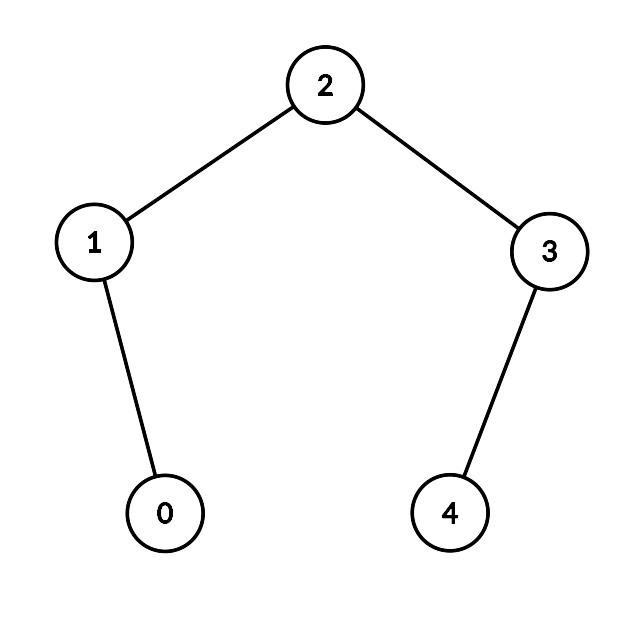
\includegraphics[height=0.15\textheight]{Figures/p5A}
		\caption{}
		\label{subfig:monotonicityA}
	\end{subfigure}
	\hfill
	\begin{subfigure}[t]{0.3\textwidth}
		\centering
		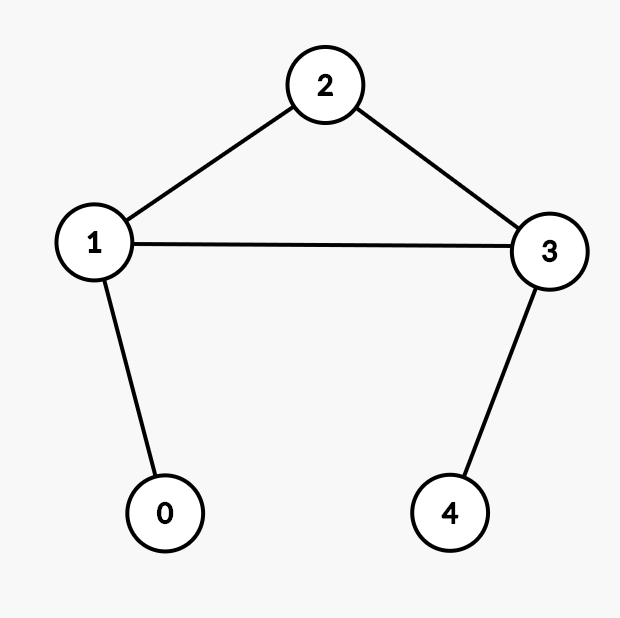
\includegraphics[height=0.15\textheight]{Figures/p5B}
		\caption{}
		\label{subfig:monotonicityB}
	\end{subfigure}
	\vspace{20pt}
	\hfill
	\caption{Edge addition between opposed opinions.}
	\label{fig:p5}
\end{figure}

\begin{equation}
	\begin{aligned}
		\\
		L+I=
		\left(\begin{matrix}
		2 & -1 & 0 & 0 & 0 \\
		-1 & 3 & -1 & 0 & 0 \\
		0 & -1 & 3 & -1 & 0 \\
		0 & 0 & -1 & 3 & -1 \\
		0 & 0 & 0 & -1 & 2
		\end{matrix}\right),
		\qquad \qquad 
		(L+I)^{-1}=
		\left(\begin{matrix}
		\frac{34}{55} & \frac{13}{55} & \frac{1}{11} & \frac{2}{55} & \frac{1}{55} \\
		\frac{13}{55} & \frac{26}{55} & \frac{2}{11} & \frac{4}{55} & \frac{2}{55} \\
		\frac{1}{11} & \frac{2}{11} & \frac{5}{11} & \frac{2}{11} & \frac{1}{11} \\
		\frac{2}{55} & \frac{4}{55} & \frac{2}{11} & \frac{26}{55} & \frac{13}{55} \\
		\frac{1}{55} & \frac{2}{55} & \frac{1}{11} & \frac{13}{55} & \frac{34}{55}
		\end{matrix}\right)
		,
		\\
		\\
		\\
		\\
		\qquad \qquad
		s=
		\left(\begin{matrix}
		-1 \\
		1 \\
		-1 \\
		-1 \\
		1
		\end{matrix}\right)
		,
		\qquad \qquad
		(L+I)^{-1}s=
		\left(\begin{matrix}
		\frac{34}{55} & \frac{13}{55} & \frac{1}{11} & \frac{2}{55} & \frac{1}{55} \\
		\frac{13}{55} & \frac{26}{55} & \frac{2}{11} & \frac{4}{55} & \frac{2}{55} \\
		\frac{1}{11} & \frac{2}{11} & \frac{5}{11} & \frac{2}{11} & \frac{1}{11} \\
		\frac{2}{55} & \frac{4}{55} & \frac{2}{11} & \frac{26}{55} & \frac{13}{55} \\
		\frac{1}{55} & \frac{2}{55} & \frac{1}{11} & \frac{13}{55} & \frac{34}{55}
		\end{matrix}\right)
		\times
		\left(\begin{matrix}
		-1 \\
		1 \\
		-1 \\
		-1 \\
		1
		\end{matrix}\right)
		=
		\left(\begin{matrix}
		\frac{-27}{55} \\
		\frac{1}{55} \\
		\frac{-5}{11} \\
		\frac{-21}{55} \\
		\frac{17}{55}
		\end{matrix}\right)
		\\
		\\
		\\
		\\
		\pi(z) = \frac{||z||_{2}^2}{n} = \frac{\sqrt{(\frac{-27}{55})^2 + (\frac{1}{55})^2 + (\frac{-5}{11})^2 + (\frac{-21}{55})^2 + (\frac{17}{55})^2}^2}{5}= 0.13785123966
	\end{aligned}
\end{equation}
\\
\\
\\
\\
We will now compute the polarization index after the addition of the edge $1\rightarrow3$.
\\
\\
\\
\begin{equation}
	\begin{aligned}
		L+I=
		\left(\begin{matrix}
		2 & -1 & 0 & 0 & 0 \\
		-1 & 4 & -1 & -1 & 0 \\
		0 & -1 & 3 & -1 & 0 \\
		0 & -1 & -1 & 4 & -1 \\
		0 & 0 & 0 & -1 & 2
		\end{matrix}\right),
		\qquad \qquad 
		(L+I)^{-1}=
		\left(\begin{matrix}
		\frac{59}{99} & \frac{19}{99} & \frac{1}{11} & \frac{8}{99} & \frac{4}{99} \\
		\frac{19}{99} & \frac{38}{99} & \frac{2}{11} & \frac{16}{99} & \frac{8}{99} \\
		\frac{1}{11} & \frac{2}{11} & \frac{5}{11} & \frac{2}{11} & \frac{1}{11} \\
		\frac{8}{99} & \frac{16}{99} & \frac{2}{11} & \frac{38}{99} & \frac{19}{99} \\
		\frac{4}{99} & \frac{8}{99} & \frac{1}{11} & \frac{19}{99} & \frac{59}{99}
		\end{matrix}\right)
		,
		\\
		\\
		\\
		\qquad \qquad
		s=
		\left(\begin{matrix}
		-1 \\
		1 \\
		-1 \\
		-1 \\
		1
		\end{matrix}\right)
		,
		\qquad \qquad
		(L+I)^{-1}s=
		\left(\begin{matrix}
		\frac{59}{99} & \frac{19}{99} & \frac{1}{11} & \frac{8}{99} & \frac{4}{99} \\
		\frac{19}{99} & \frac{38}{99} & \frac{2}{11} & \frac{16}{99} & \frac{8}{99} \\
		\frac{1}{11} & \frac{2}{11} & \frac{5}{11} & \frac{2}{11} & \frac{1}{11} \\
		\frac{8}{99} & \frac{16}{99} & \frac{2}{11} & \frac{38}{99} & \frac{19}{99} \\
		\frac{4}{99} & \frac{8}{99} & \frac{1}{11} & \frac{19}{99} & \frac{59}{99}
		\end{matrix}\right)		\times
		\left(\begin{matrix}
		-1 \\
		1 \\
		-1 \\
		-1 \\
		1
		\end{matrix}\right)
		=
		\left(\begin{matrix}
		\frac{-53}{99} \\
		\frac{-7}{99} \\
		\frac{-5}{11} \\
		\frac{-29}{99} \\
		\frac{35}{99}
		\end{matrix}\right)
		\\
		\\
		\\
		\pi(z) = \frac{||z||_{2}^2}{n} = \frac{\sqrt{(\frac{-53}{99})^2 + (\frac{-7}{99})^2 + (\frac{-5}{11})^2 + (\frac{-29}{99})^2 + (\frac{35}{99})^2}^2}{5} = 0.14180185695
	\end{aligned}
\end{equation}
\\
We can see an increase of the polarization index after adding this particular edge. This example was discovered after brute-forcing different graph topologies with different combinations of opinion values.
\\	
\begin{lemma}
The polarization index does not necessarily decrease after an edge addition between opposing views.
\end{lemma}

\section{Polarization in a complete graph}
\label{sec:fullgraph}
\vspace{20pt}
Given a polarized graph $G$ we will compute the polarization index $\pi(z)$ before and after converting the graph $G$ to a full graph. 

\begin{table}[!htb]
 \centering
 \caption{Polarization Before and after converting to a full graph}
 \label{tab:fullgraph}
 \begin{tabular}{| l || l | l | l | l |}
 \hline
  Dataset & Number of Nodes & Number of edges & Average Degree & $\pi(z)$\\
  \hline
  \hline
  Karate Before & $34$ & $78$ & $4.5882$ &  $0.35857$\\
  \hline
  Karate After & $34$ & $561$ & $33$ &  $0.00081$\\
  \hline
  \hline
  Books Before & $105$ & $441$ & $8.4000$ &  $0.44046$\\
  \hline
  Books After & $105$ & $5460$ & $104.0000$ &  $0.00453$\\
  \hline
  \hline
  Blogs Before & $1490$ & $16718$ & $22.4403$ &  $0.27909$\\
  \hline
  Blogs After & $1490$ & $1109308$ & $1489.0040$ &  $0.00030$\\
  \hline
 \end{tabular}
 \end{table}

\vspace{20pt}
We can see the results from the karate, books and blogs datasets at table ~\ref{tab:fullgraph} The results leads us to the following lemma.
\\	
\begin{lemma}
The polarization index does not drop to zero in a fully connected graph.
\end{lemma}

